%%%%%%%%%%%%%%%%%%%%%%%%%%%%%%%%%%%%%%%%%
% Journal Article
% LaTeX Template
% Version 1.4 (15/5/16)
%
% This template has been downloaded from:
% http://www.LaTeXTemplates.com
%
% Original author:
% Frits Wenneker (http://www.howtotex.com) with extensive modifications by
% Vel (vel@LaTeXTemplates.com)
%
% License:
% CC BY-NC-SA 3.0 (http://creativecommons.org/licenses/by-nc-sa/3.0/)
%
%%%%%%%%%%%%%%%%%%%%%%%%%%%%%%%%%%%%%%%%%

%----------------------------------------------------------------------------------------
%	PACKAGES AND OTHER DOCUMENT CONFIGURATIONS
%----------------------------------------------------------------------------------------

\documentclass[twoside,twocolumn]{article}

\usepackage{blindtext} % Package to generate dummy text throughout this template 

\usepackage[sc]{mathpazo} % Use the Palatino font
\usepackage[T1]{fontenc} % Use 8-bit encoding that has 256 glyphs
\linespread{1.05} % Line spacing - Palatino needs more space between lines
\usepackage{microtype} % Slightly tweak font spacing for aesthetics

\usepackage[english]{babel} % Language hyphenation and typographical rules

\usepackage[hmarginratio=1:1,top=32mm,columnsep=20pt]{geometry} % Document margins
\usepackage[hang, small,labelfont=bf,up,textfont=it,up]{caption} % Custom captions under/above floats in tables or figures
\usepackage{booktabs} % Horizontal rules in tables

\usepackage{lettrine} % The lettrine is the first enlarged letter at the beginning of the text

\usepackage{enumitem} % Customized lists
\setlist[itemize]{noitemsep} % Make itemize lists more compact

\usepackage{abstract} % Allows abstract customization
\renewcommand{\abstractnamefont}{\normalfont\bfseries} % Set the "Abstract" text to bold
\renewcommand{\abstracttextfont}{\normalfont\small\itshape} % Set the abstract itself to small italic text

\usepackage{titlesec} % Allows customization of titles
\renewcommand\thesection{\Roman{section}} % Roman numerals for the sections
\renewcommand\thesubsection{\Roman{section} \Alph{subsection}} % roman numerals for subsections
\titleformat{\section}[block]{\large\scshape\centering}{\thesection.}{1em}{} % Change the look of the section titles
\titleformat{\subsection}[block]{\large}{\thesubsection.}{1em}{} % Change the look of the section titles

\usepackage{fancyhdr} % Headers and footers
\pagestyle{fancy} % All pages have headers and footers
\fancyhead{} % Blank out the default header
\fancyfoot{} % Blank out the default footer
\fancyhead[C]{State of Art of Artificial Neurals Networks Compression} % Custom header text
\fancyfoot[RO,LE]{\thepage} % Custom footer text

\usepackage{titling} % Customizing the title section

\usepackage{hyperref} % For hyperlinks in the PDF

\usepackage{amsmath,array}
\newcommand*{\vertbar}{\rule[-1ex]{0.5pt}{2.5ex}}
\newcommand*{\horzbar}{\rule[.5ex]{2.5ex}{0.5pt}}

\usepackage{graphicx}
\graphicspath{ {./images/} }
%----------------------------------------------------------------------------------------
%	TITLE SECTION
%----------------------------------------------------------------------------------------

\setlength{\droptitle}{-4\baselineskip} % Move the title up

\pretitle{\begin{center}\Huge\bfseries} % Article title formatting
\posttitle{\end{center}} % Article title closing formatting
\title{State of Art in Artificial Neurals Networks Compression} % Article title
\author{%
\textsc{Pierre Gabin FODOP GUMETE} \\[1ex] % Your name
\normalsize ENSTA Bretagne \\ % Your institution
\normalsize \href{mailto:pierre.fodop@ensta-bretagne.org}{pierre.fodop@ensta-bretagne.org} % Your email address
%\and % Uncomment if 2 authors are required, duplicate these 4 lines if more
%\textsc{Jane Smith}\thanks{Corresponding author} \\[1ex] % Second author's name
%\normalsize University of Utah \\ % Second author's institution
%\normalsize \href{mailto:jane@smith.com}{jane@smith.com} % Second author's email address
}
\date{\today} % Leave empty to omit a date
\renewcommand{\maketitlehookd}{%
\begin{abstract}
  Les vingt dernières années ont vu une augmentation exponentielle de la puissance de calcul des ordinateurs personnels,
  en plus de l'explosion des services de cloud et l'augmentation du nombre de fermes à serveurs pour le stockage de données. 
  Cette Augmentation a eu parmi ses conséquences de mettre à la disposition du plus grand nombre un certain nombre de 
  données, mais aussi l'explosion des méthodes de Réseaux de neurones. Ils ont été appliqués à un nombre important de problèmes 
  notamment en traitement d'image, traitement du son, en traitement du langage naturel (...) Domaines dans lesquels ils 
  constituent à ce jour l'état de l'art. D'un autre côté, on a aussi eu une progression importante de l'Internet des Objets, cela 
  a créé le besoin de reseaux de neurones adaptés aux objets peut puissant. L'objectif de ce papier est de présenter les différentes 
  methodes permettant de compresser les réseaux de neurones et par là de stocker les réseaux dans un moindre espace, mais aussi 
  d'accélérer les calculs avec ces derniers.
\end{abstract}
}

%----------------------------------------------------------------------------------------

\begin{document}

% Print the title
\maketitle

%----------------------------------------------------------------------------------------
%	ARTICLE CONTENTS
%----------------------------------------------------------------------------------------

\section{Introduction}
L'Histoire des réseaux de neurones débute avec Warren S. McCulloch et Walter Pitts de chercheurs du MIT qui présentent 
en 1943 un article sur la réalisation des fonctions neuronales par des fonctions électriques et des portes logiques\cite{warren1}.
Leur approche est lié à une perception des fonctions neuronales comme des fonctions {\bf\textit{Tout ou rien}}. Cette avancée 
sera complete plus tard par la définition du perceptron\cite{RosenBlatt1} et la decouverte de l'algorithme de retro-propagation 
du gradiant\cite{Rumelhart1}.

\begin{figure}[h]
\centering
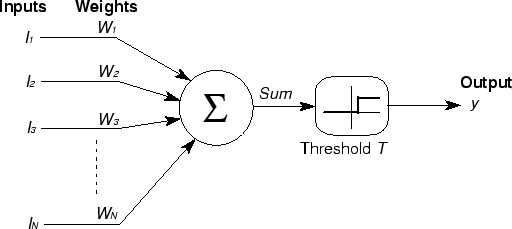
\includegraphics[width=70mm]{CulochNeurone.png}
\caption{Modèle Calculatoire de McCulloch et Pitts}
\label{SimpleNeuron}
\end{figure}

L'\textit{hivers de l'Intelligence arrtificielle} qui commencera à la fin de la décennie 1960 les avancées dans le domaine de l'intelligence artificielle
se font plus lentes. À cause d'une réduction des investissements autant publique que privée dans le domaine. Bien que ralenti, c'est dans cette période que
sont conçu les premières implémentations à grande échelle des systèmes expert conçu en 1950. Ici la majeur partie des systèmes intelligents fonctionnes avec une 
base dite \textit{Knowlege Based}(Basé sur la connaisance). On a donc un développement des bases de methodes telque la Programation Logique Inductive (ILP)
\cite{Muggleton1}\cite{Ehud1}. Qui sera plus tard compilé par S.H. Muggleton dans son artice fondateur "Inductive Logic Programming"\cite{Muggleton2}.

Enfin, dans les années 1990, on a un retour en force des méthodes d'intelligence artificielle avec l'augmentation de la puissance de calcul ; cela avec l'avènement
des premiers processeurs Pentium par Intel, une généralisation des super calculateurs et enfin l'avènement d'Internet qui permettra un échange de connaissance
sans précèdent. Cette évolution atteindra un premier grand pallié en 2012 avec l'application des réseaux de neurones au challenge de classification d'image ImageNet
qui permettra de faire passer le taux le plus faible d'erreur de classification de 25\% a 16\% grace au réseau AlexNet\cite{Rajat1}. 

Depuis lors, les réseaux de neurones ont été appliqués à un nombre de plus en plus grand de problème. Notement en Vision par ordinateur\cite{MadhusmitaSahu}
\cite{Sornaminproceedings}, en traitement du langage naturel\cite{jing2019survey}, en analyse des signaux\cite{MohamedIbn1}\cite{XiaofanLi1} et bien d'autres
\cite{POZNYAK2019250} Avec des resultats meilleurs que les méthodes qui etaient utilisé jusque là. Ceci a crée le besoin de réseaux de neurones adapté à un certain 
nombre de supports. Notamment les supports issue de L'Internet des Objets. 

L'objectif de ce document est de faire un tour des méthodes permettant de compresser des réseaux de neurones et de les appliques dans un certain nombre d'objets, 
pour ce faire, nous commencerons par faire une présentation des différentes architectures de réseaux de neurones existantes, en suite, nous explorerons les méthodes 
de pruning, de représentation creuse notamment quantifie, de distillation de connaissance et enfin, nous verrons les méthodes futures 

%------------------------------------------------

\section{Types de Réseaux de Neurones}

\subsection{Le Perceptron}

C'est l'expression la plus simple d'un réseau de neurones, il est constitué d'un seul neurone formel\cite{warren1}.

\begin{figure}[h]
  \centering
  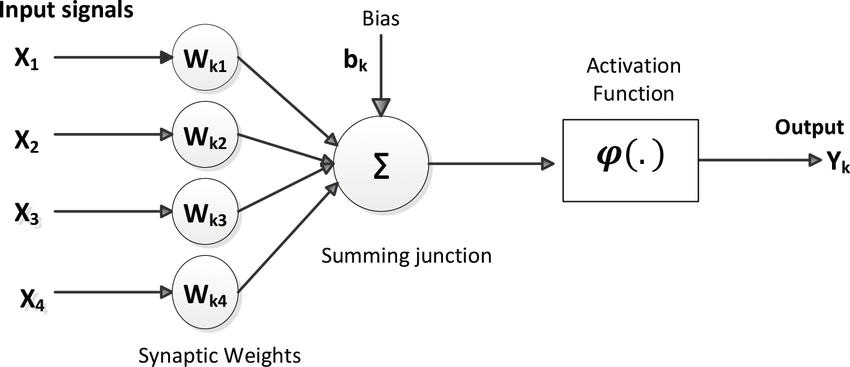
\includegraphics[width=70mm]{McCulloch-Pitts-computational-model-of-a-neuron.png}
  \caption{Perceptron Multi-Couche}
  \label{PerceptronMathematique}
\end{figure}

Le neurone prend en entrée un vecteur de valeur $x$, le multiplie par un vecteur de poids $w$ enfin grace a la fonction d'activation
nous retourne la sortie.
\[
y = \varphi(
\left[
  \begin{array}{ccc}
    w_{1}\\
    w_{2}\\
    w_{3}\\
    w_{4}\\  
  \end{array}
\right]*
\begin{bmatrix}
           x_{1} \\
           x_{2} \\
           x_{3} \\
           x_{4}
         \end{bmatrix}
+ b)\]
La fonction d'activation $\varphi()$ doit remplir un certain nombre de condition.
\begin{itemize}
  \item \textbf{L'identite en zero} si $f(x) = 0$ alors $x = 0$ \cite{Sussillo2014RandomWI} Ces fonctions permettent de faire un apprentissage rapide.
  \item \textbf{Derivee de valeur monotone}\cite{WU20093432} pour une meilleur capacite de generalisation et une facilite d'application des methodes d'optimisation convexe.
  \item \textbf{Partout Differentiable}\cite{Rumelhart1} permetant l'application de la descente de gradiant.
\end{itemize}

Pour mettre a jour les poids $w$ de notre perceptron, nous utiliseron l'algorithme de descente de gradient. Ce dernier permet a partir d'une fonction d'erreur choisie, de faire
une mise a jour de ces poids.
Soit $F(x)$ une fonction definie et differentiable au voisinage du point $a$ minimum local. L'objectif etant d'estimer la valeur de a; on definira un coeficient d'aprentissage $\lambda$.
On definira donc la suite suivante avec une intitialisation a $a_0$. 

\[\left\{
  \begin{array}{rcr}
    a_{0} & =  a_0 \\
    a_{n+1} & = & a_{n} - \lambda. \Delta F(a_n)\\
  \end{array}
\right.\]

Pour un reseau de neurone avec comme fonction d'activation la sigmiode et comme fonction d'erreur la fonction \textit{cross entropy loss}

$E(y) = -(y^v.log(y) + (1-y^v).log(1-y))$
\[ \frac{\partial E}{\partial w}
   = \frac{\partial E}{\partial y}
   *\frac{\partial y}{\partial z}
      *\frac{\partial z}{\partial w}\]

\[ \frac{\partial E}{\partial y}
  =  \frac{y^v}{y} - \frac{1-y^v}{1-y}
  = \frac{y^v - y}{y(1 - y)} \]

\[ \frac{\partial y}{\partial z}
  =  y*(1-y) \]

\[ \frac{\partial z}{\partial w}
  =  w^T \]

\[ \frac{\partial E}{\partial w}
  = x*(y^v-y) \]

d'ou on a 
\[\left\{
  \begin{array}{rcr}
    w_{0} & =  w_0 \\
    w_{n+1} & = & w_{n} - \lambda.(y^v-y).x\\
  \end{array}
\right.\]
la procedure est identique pour la mise a jour des biais.

A sa sortie,un neurone permet de faire une classification d'une classe en deux classe de valeurs. 
Celles qui actives le neurones et celles qui ne l'activent pas; on peut en utiliser plusieurs pour 
faire des classifications dans un nombre de classes plus important. On obtiendra alors des perceptron
multi-couche

\subsection{Les perceptrons Multi-Couches}
C'est le type de reseaux de neurones le plus basique, il est constitue d'un certain nombre de couche elle meme constitue de de neurone formel\cite{warren1}. 
Les informations sont ainsi tansmises de la premieres couche dite couche d'entree a la dernieres couche dite de sortie en passant par les couches cache au travers
de connection entre les neurones. Au cas ou chaque neurone d'une couche est lie a tous les neurones de la couche suivante on parle de reseaux entierement connectes,

\begin{figure}[h]
  \centering
  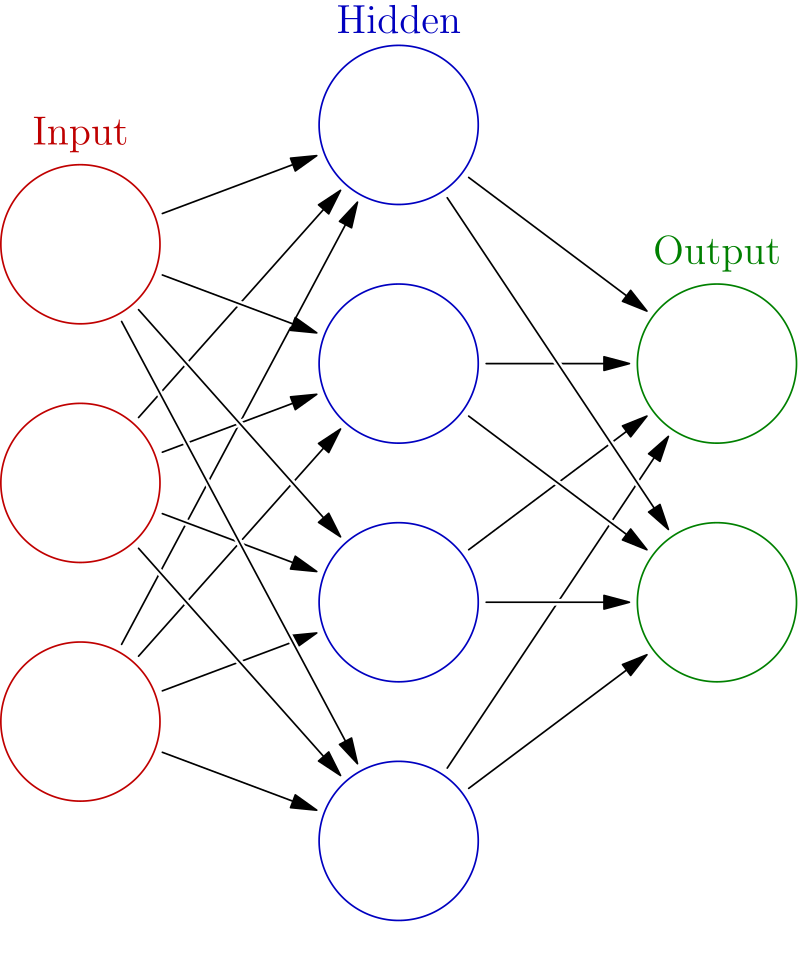
\includegraphics[width=60mm]{Colored_neural_network.png}
  \caption{Perceptron Multi-Couche}
  \label{PerceptronMulticouche}
  \end{figure}

Actuellement, les perceptrons multi-couches, obtiennent dans les meilleures conditions un taux d'erreur inferieure a 0.35\%.\cite{DeepBig} L'equivalent mathematique d'un resaux a 784 neurones d'entree 16 caches et 10 de sortie est le suivant:

\[
y^1 = \varphi_1(
\left[
  \begin{array}{ccc}
    w_{1}^{1} & ... & w_{1}^{784}\\
    \vdots & \vdots & \vdots\\
    w_{16}^{1} & ... & w_{16}^{784}\\  
  \end{array}
\right]*
\begin{bmatrix}
           x_{1} \\
           \vdots \\
           x_{784}
         \end{bmatrix}
+ \begin{bmatrix}
  b_{1} \\
  \vdots \\
  b_{784}
\end{bmatrix}
)\]

\[
y^2 = \varphi_2(
\left[
  \begin{array}{ccc}
    w_{1}^{1} & ... & w_{1}^{16}\\
    \vdots & \vdots & \vdots\\
    w_{10}^{1} & ... & w_{10}^{16}\\  
  \end{array}
\right]*
\begin{bmatrix}
           x_{1} \\
           \vdots \\
           x_{10}
         \end{bmatrix}
+ \begin{bmatrix}
  b_{1} \\
  \vdots \\
  b_{10}
\end{bmatrix}
)\]
Pour faire une distribution probabilistique des sorties, nous pouvonts utiliser un certaint nombre de fonction, dans ce cas, nous utiliserons 
Une fonction softmax.
\[
out = softmax(y^2)
\]
on aura donc un verceur de 10 probabilites, qui signifient chacune si la classe represente est la classe adequate.


\subsection{Les Reseaux de Neurones Convolutionnel (CNN)}
%------------------------------------------------
Le plus grand defaut des reseaux de type perceptron multi couche est leur incapcite a traiter une image en tant qu'information globale a conduit au developpement des
reseaux de neurones Convolutionnel.

Le filtrage pour une image est une operation mathematique qui permet a base d'une matrice appele kernel de faire un certain nombre d'operation sur une image. On peut citer parmi ces derniere le floutage,
la detection de contour. Cela se fera par convolution d'une matrice appelle noyau avec une notre image. sa representation mathematique est la suivante:
\[g(x,y) = w*f(x,y)\]
\[w*f(x,y) = \sum_{dx=-a}^{a} \sum_{dx=-b}^{b} w(dx,dy)f(x+dx,y+dy)\]

Dans le cadre de la detection de contour qui est une des base des reseaux de neurones convolutionnel, On utilisera de facon preferentiel du filtrage de Canny \cite{Canny1}

\begin{figure}[h]
  \centering
  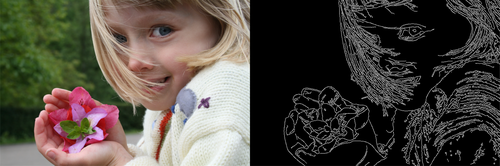
\includegraphics[width=60mm]{canny.png}
  \caption{Filtrage de Canny}
  \label{CannyOutput}
  \end{figure}

Pour une couche convolutionnelle, nous appliquerons a notre image un certain nombre de filtre convolutionnel qui permetrons de saisir un maximum d'information sur l'image. Nous pourons appliquer un Pooling sur les image filtees obtenu pour en reduire le nombre de dimenssion.

\begin{figure}[h]
  \centering
  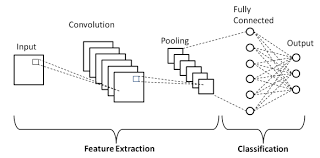
\includegraphics[width=72mm]{convneural.png}
  \caption{Reseau Convolutionnel}
  \label{ConvNet}
\end{figure}
Et a la fin du reseau, nous appliquerons un reseau de type Multi layer perceptrons pour classifier les images. Il est aussi possible d'avoir un reseau entierement convolutionnel.

Les application des reseaux de types convolutionnels sont nombreuses, autant en traitement d'image \cite{Browne1} (VGG16, LeNet, ...), qu'en traitement du langage naturel\cite{8666928}, ou en traitement des signaux audios\cite{Gama_2019}. 
Bien que les reseaux de neuronnes convolutionnels completent les reseaux perceptron, ils presentent la limite de ne pas prendre en compte des valeurs temporelle et sont assez peux utiles pour annalyser des sequences tels que des sequence video.
\subsection{Recurent Neural Network}
Les reseaux recurents, on ete cree pour permettre un transfert de l'information dans les cellules en prenant en compte l'infulence du temps. 
Ici on parle d'une double propagation spaciaux temporelle. Cela donne la capacite a ces neuronnes d'intervenir dans l'analyse des phenomene evoluant dans le temps comme les videos, les series temporelles ...

Les reseaux recurents on vu le jour avec le reseau de Hopfield\cite{Hopfield}. Ce dernier introduit la memoire dans les reseau permetant un passage au traver le temps des informations.Ils connaitrons quelques evolutions jusqu'a l'arive d'un autre type 
de reseaux de neurone, Le \textit{Long Short Term Memory}\cite{lstm1}

\begin{figure}[h]
  \centering
  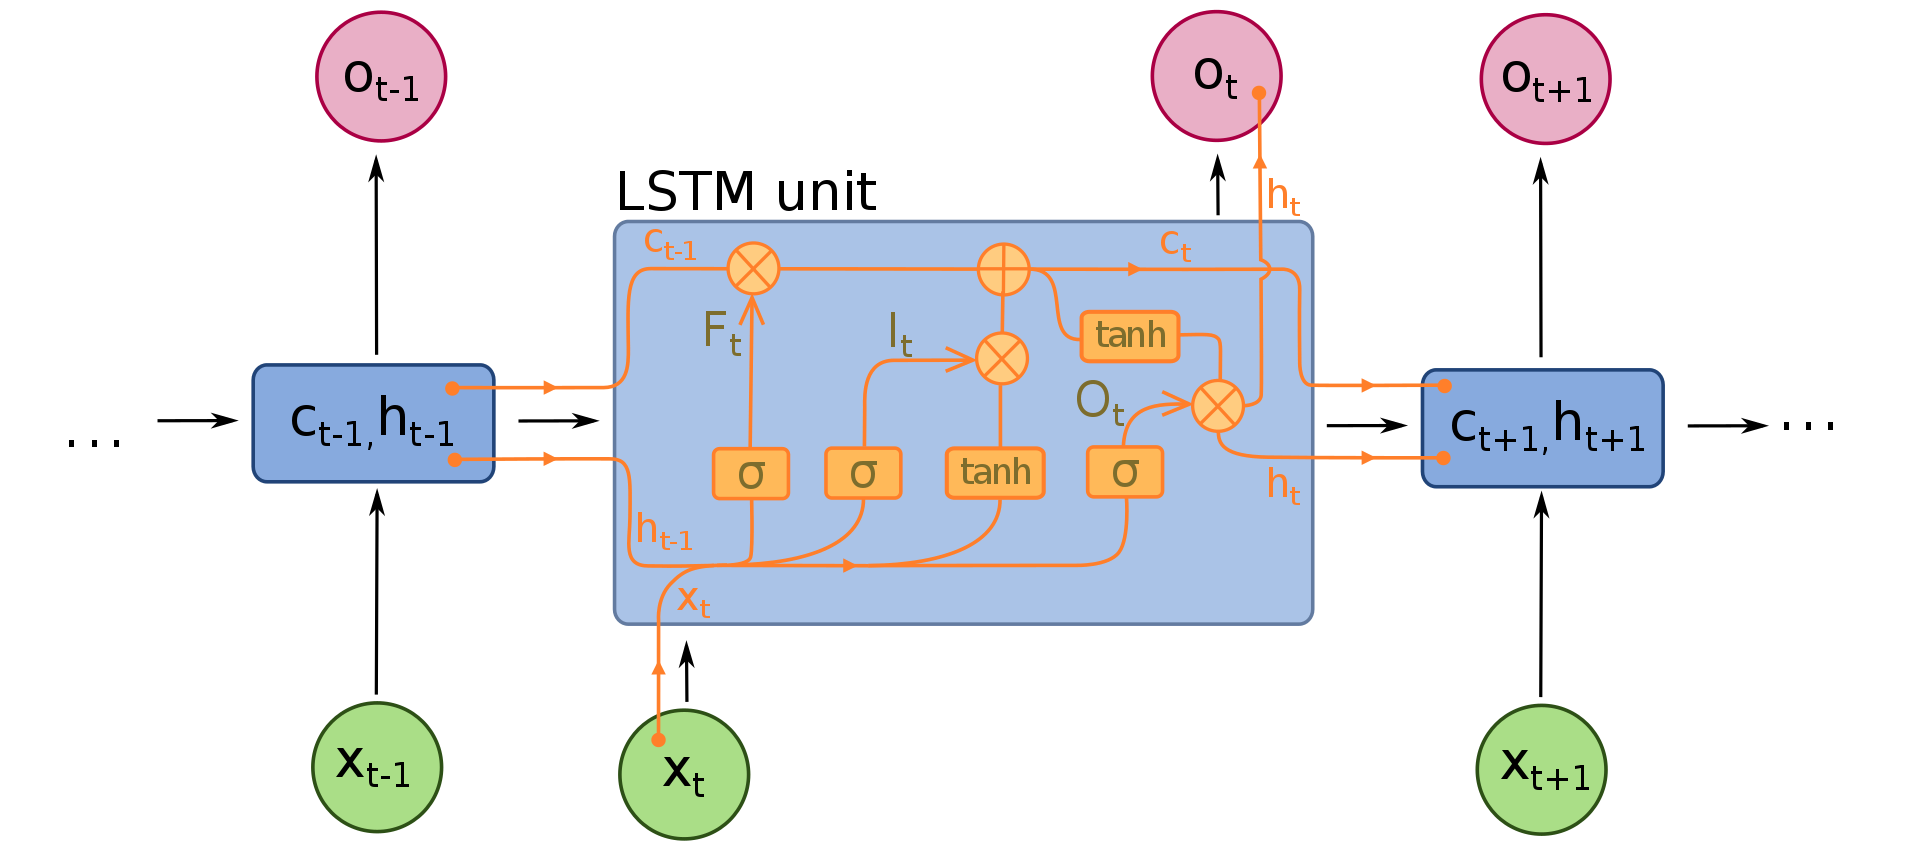
\includegraphics[width=72mm]{Long_Short-Term_Memory.png}
  \caption{Cellule LSTM}
  \label{lstm}
\end{figure}

Une celule LSTM prend en entree 3 valeurs valeurs, les sorties de la celule precedente $H_t$ l'etat cache et $C_t$ l'etat de la celule; mais aussi la valeur actuelle d'entree $X_t$. 

la premiere porte que nous verons est porte de l'oublie. la fonction de la porte d'oublie est la suivante:
\[f_t = \sigma(U^fX_t + W^fh_{t-1})\]
Les portes suivantes permettent de calculer l'etat d'entree et l'etat de sortie
\[i_t = \sigma(UX_t + Wh_{t-1})\]
\[O_t = \sigma(U^{\circ}X_t + W^{\circ}h_{t-1})\]
La porte de sortie
\[g_t = tanh(U^gX_t + W^gh_{t-1})\]
etat final de la cellule
\[c_t = i_tg_t + f_tc_{t-1}\]
Et l'etat cache suivant
\[h_t = tanh(c_t)o_t\]

Enfin en 2014 seront introduit les celule dites Gated Recurrent Unit (GRUs)\cite{cho2014learning}. 

\begin{figure}[h]
  \centering
  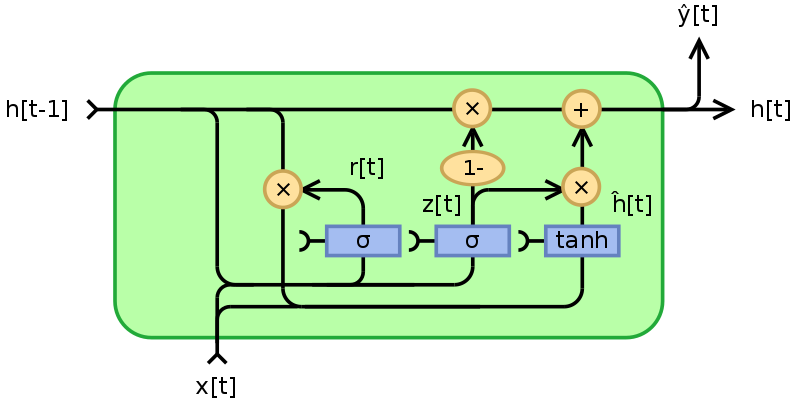
\includegraphics[width=70mm]{GRU.png}
  \caption{Cellule GRU}
  \label{GRUs}
\end{figure}

La cellule GRU prend en entre 2 variables et genere deux sorties. Les entrees sont $h_t$ l'etat cache provenant de la precedente cellule 
$x_t$ la valeur actuelle de l'entree ; les sorties sont quant a elles, $y^est$ la valeur de sortie estimee et $h_t$ l'etat cache estime.

Du point de vue mathematique on a:
\[z_t = \sigma_g(W_{z}x_{t} + U_{z}h_{t-1} + b_{z})\]
\[r_t = \sigma_g(W_{r}x_{t} + U_{r}h_{t-1} + b_{r})\]
\[h_{t}^{est} = \phi_h(W_{h}x_{t} + U_{h}(r_t * h_{t-1}) + b_{h})\]
\[h_t = (1 - z_t)*h_{t-1} + z_t*h_{t}^{est}\]
ou $x_t$ est le vecteur d'entree, $h_t$ le vecteur de sortie, $z_t$ le vecteur de mise a jour des protes, $r_t$ vecteur de reinitialisation, $h_t^{est}$ Vecteur candidat d'acivaion.
$W$, $U$ et $b$ sont les marices de parametre. $\sigma_g$ est la fonction sigmoide et $\phi_h$ est la tangente hyperbolique.

Plus recement, les GRU ont ete modifie pour donner les reseaux Minimal Gated Unit \cite{heck2017simplified}\cite{zhou2016minimal}. Ces reseaux presentent l'avantage d'avoir un minimum
d'entree de sortie et de porte logiques.

\begin{figure}[h]
  \centering
  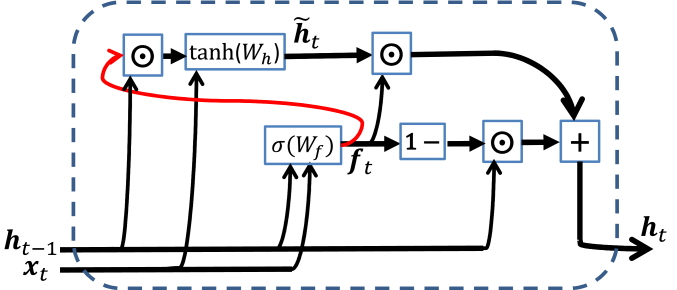
\includegraphics[width=70mm]{MRU.png}
  \caption{Cellule MRU}
  \label{MRUs}
\end{figure}

\subsection{Autres reseaux}
Les types de reseaux de neurones presente plus haut on tous la particularite d'etre en apprendtissage supervise. Ce genre  de reseaux est generalement utilise pour la classification.
Dans cette partie nous nous interesserons au cas des autres types de reseaux dont l'apprentissage est generalement non supervisee. 

les premiers de ces reseaux seront, \textbf{Les Machines de Bolztmann}. l'origine de ces reseaux est l'article de Hinton et Sejnowski de 1983\cite{Rumelhart2}, ils sont utilise pour avoir des estimation de distribution
probabiliste d'un jeux de donnee\cite{Salakhutdinov}. Ces derniers sont generalement utilise sous la forme de machine de bolzmann restreinte a deux couches de neurones. 

En suite nous avons les \textbf{chaines de Markov}, Il s'ait ici d'un reseaux qui a base de connaisance de l'etat actuelle et d'un ensemble de probabilite connue peut predire les etat futur. Elles sont utilise sur les 
processus a temps discret, ou a temps continu et a espace d'etats discret.

Enfin nous classeron un certain nombre de reseaux notemment les auto encodeur (auto-encodeur variationnel, auto encodeur de debruitage), les Reseaux generatifs adversariaux (...) dans la cathegorie des reseaux composees
en cela qu'il sont issue de la composition d'un certain nombre de couche de neuronne issue des reseaux mentionne plus haut.

\section{Pourquoi la compression des reseaux de neurones}%----------
L'origine des objets connectes remonte a 1994 quand la start-up Violet a lance le concept de la lampe connecte en wifi DAL. Et depuis lors leur nombre n'a pa arrete de croitre, leur usage aussi. D'un autre cote le nombre d'outils 
informatique a lui aussi augmente de facons considerable, avec l'invention des smartphones, des tabletes et autres.

Ces objets connnectes ont pour point commun de ne disposer ni d'une grande puissance de calcul ni d'un grand espace de stockage. Cette situation les eloignes des possiblite d'aplication des reseaux de neurones qui quand a eu on besoin
d'une puissance de calcule importante et d'un espace de stockage lui aussi grand.

\begin{table}[!h]  
\begin{tabular}{|l|c|r|}
    \hline
    DNN & Size(MB) & Temps(Milion) \\
    \hline
    AlexNet & 200 & 720 \\
    VGG-16 & 550 & 15 300 \\
    GoogLeNet & 50 & 1550 \\
  ResNet & 170 & 11 300 \\
  \hline
\end{tabular}
\caption{Les Poids et temps de calcul de differents reseaux}
\end{table}

Pour rendre ces objet plus intelligent il est donc important pour nous de pouvoir developper des reseaux de neurones adaptés. Pour ce faire, 
un certain nombre de moyens et de methodes ont ete developpe. Parmi les methodes qui s'attaquent a reduire le poid des reseaux on a, Le pruning, la quantification, la distillation de connaisance.
D'autres approches visent une repartition des calclus entre plusieurs objets comme l'apprentissage federe. Nous explorerons ici en profondeur les approches qui 
s'attellent a reduire la taille des reseaux et nous ferons une introduction de l'aprentissage federe. Enfin , Dans la mesure ndu possible, nous presenterons les resultas que nous avons eu en 
modelisant les methodes.

\section{Le Pruning} %-------------------------------

\subsection{C'est quoi le Pruning}
L'une des premieres idee pour reduire la taille des reseaux en memoire, est de suprimer les connections inutiles entre les neurones.
En effet lors de l'entrainement des reseaux de neurones et leur utilisation, ils existent potentiellement des connections qui se sont jamais 
activee, leurs supression  fait donc gagner de l'espace de stockage.

Le Pruning est la methode de reduction de taille des reseaux de neurones qui consiste a suprimer les poids inferieure a un certain seuil.

\begin{figure}[h]
  \centering
  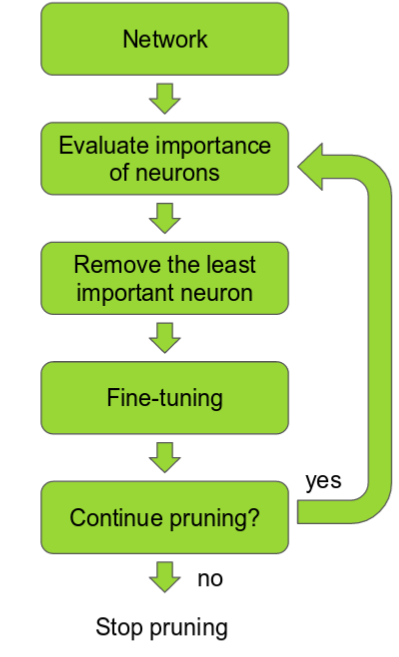
\includegraphics[width=40mm]{pruning_steps.png}
  \caption{etapes de Pruning}
  \label{Pruning_step}
\end{figure}

\begin{figure}[h]
  \centering
  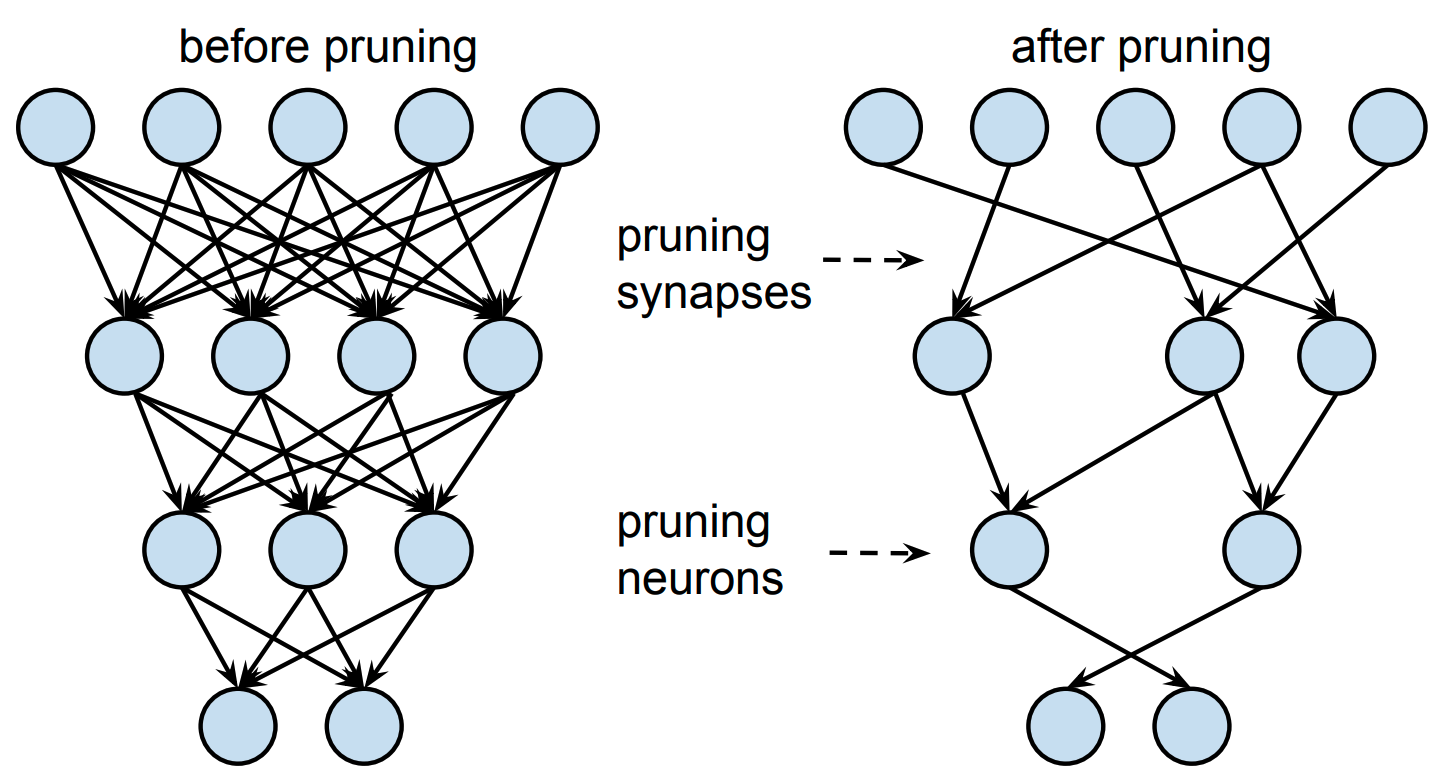
\includegraphics[width=70mm]{pruning.png}
  \caption{Pruning}
  \label{pruning du perceptron Multicouche}
\end{figure}
Les recherches dans ce dommaine sont oriente vers la resolution du probleme compression/ efficacite qui en decoule. 

Dans la section qui suit, nous presenterons l'etat de l'art de la methode de pruning cela en nous  attardant sur certaines publications
que nous avons selectionnee.

\subsection{Etat de l'art de la methode Pruning}
La premiere publication majeure qui a pose les jalon de l'application de la methode de pruning nous date des annee 1991\cite{SYKung}. l'idee principale de ce dernier est 
d'utiliser le mean square error associer a la norme de Forbenius pour 

\subsection{Le futur du Pruning}
\subsection{Presentation de mes resultats}

\section{Quantification}%---------------------
\subsection{Quantification}
\subsection{Binarization}

\section{Distillation de connaissance} %--------------


\section{Autres Methodes}%-----------


\section{Conclusion}%---------

%----------------------------------------------------------------------------------------
%	REFERENCE LIST
%----------------------------------------------------------------------------------------

\bibliographystyle{plain}
\bibliography{reference} 

%----------------------------------------------------------------------------------------

\end{document}
